\documentclass[tikz,border=25pt]{standalone}
\usepackage{fontspec}\setmainfont{Arial}
\usepackage{pgfplots,ifthen,etoolbox}
\pgfplotsset{compat=newest,compat/show suggested version=false}
\usetikzlibrary{positioning,calc}
\newlinechar=`\^^J

\newcommand{\MOVE}[2]{
 \ifdimless{15.0pt}{#1pt}{%
  \pgfmathtruncatemacro#1{0}
  \pgfmathparse{#2-7}
  \pgfmathtruncatemacro#2{\pgfmathresult}
 }{
 \pgfmathparse{#1+5}
 \pgfmathtruncatemacro#1{\pgfmathresult}
 }
}

\begin{document}
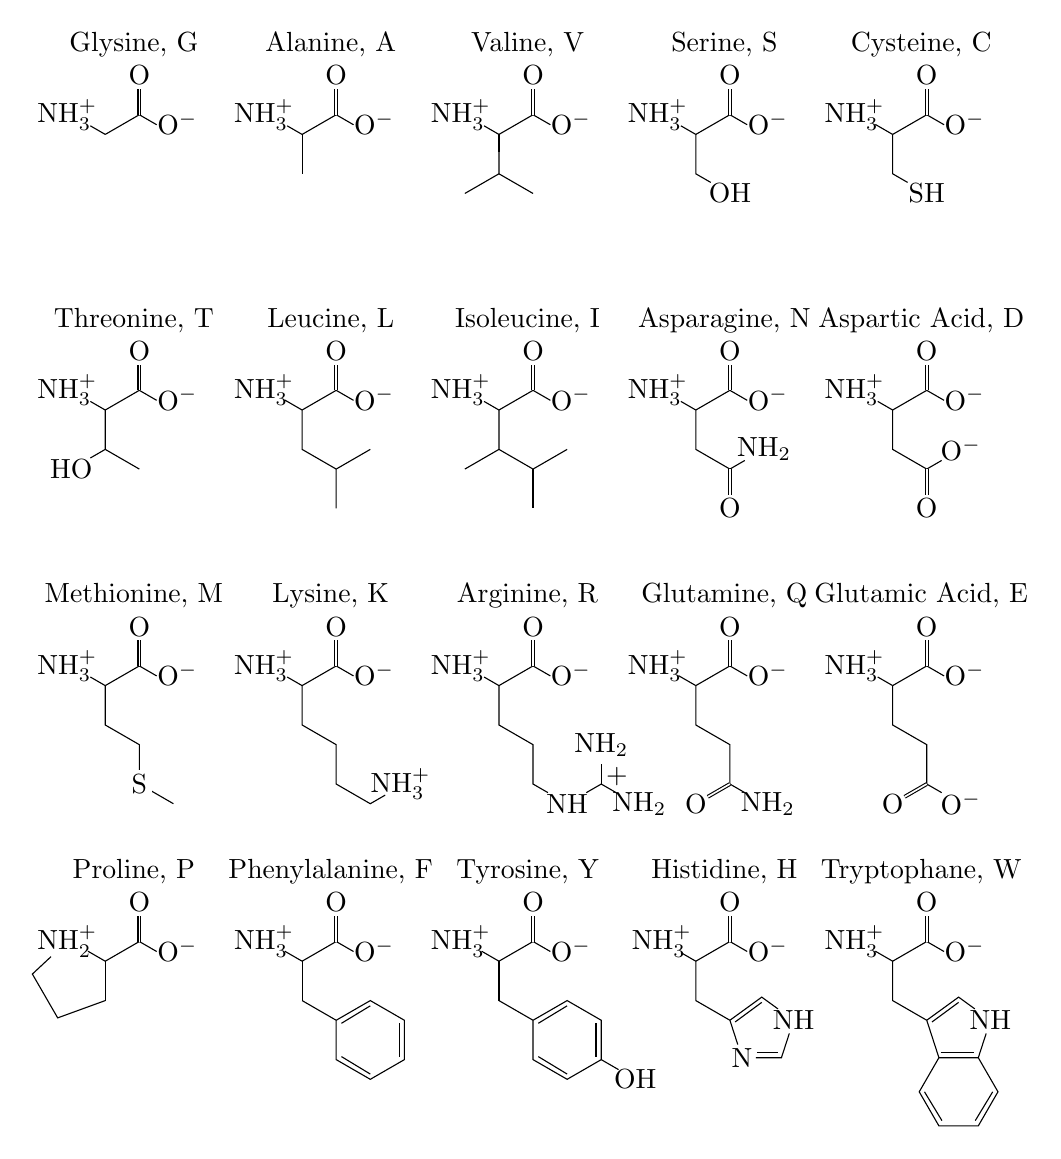
\begin{tikzpicture}
\tikzstyle{every node}=[inner sep=1.7pt,anchor=center]
\tikzstyle{to_1}=[shorten >=5pt,double]
\tikzstyle{to_2}=[shorten >=7pt]
\tikzstyle{to_3}=[shorten >=8pt]
\tikzstyle{from_1}=[shorten <=5pt]
\tikzstyle{from_1i}=[shorten <=6pt]
\tikzstyle{from_2}=[shorten <=8pt]
\edef\col{0}
\edef\line{0}

\begin{scope}[scale=0.5]
 \coordinate(CA)at(\col,\line);
 \draw[to_2](CA.center)
  --++(30:1)node(CO){}  
  --++(330:1)node[anchor=base,xshift=0.5mm]{O$^{-}$};
 \draw[to_1,double](CO.center)
  --++(90:1)node(Od){O};
 \draw[to_3](CA.center)
  --++(150:1)node[xshift=-0.5mm]{NH${_{3}^{+}}$};
 \node[above=0.6cm of CO,xshift=-0.7mm]{Glysine, G};
\end{scope}

\MOVE{\col}{\line}

\begin{scope}[scale=0.5]
 \coordinate(CA)at(\col,\line);
 \draw[to_2](CA.center)
  --++(30:1)node(CO){}  
  --++(330:1)node[anchor=base,xshift=0.5mm]{O$^{-}$};
 \draw[to_1,double](CO.center)
  --++(90:1)node(Od){O};
 \draw[to_3](CA.center)
  --++(150:1)node[xshift=-0.5mm]{NH${_{3}^{+}}$};
 \draw(CA.center)
  --++(270:1)node(Cb){};
 \node[above=0.6cm of CO,xshift=-0.7mm]{Alanine, A};
\end{scope}

\MOVE{\col}{\line}

\begin{scope}[scale=0.5]
 \coordinate(CA)at(\col,\line);
 \draw[to_2](CA.center)
  --++(30:1)node(CO){}  
  --++(330:1)node[anchor=base,xshift=0.5mm]{O$^{-}$};
 \draw[to_1,double](CO.center)
  --++(90:1)node(Od){O};
 \draw[to_3](CA.center)
  --++(150:1)node[xshift=-0.5mm]{NH${_{3}^{+}}$};
 \draw[to_3](CA.center)
  --++(270:1)node(Cb){};
 \draw(CA.center)
  --++(270:1)node(Cb){}
  --++(330:1)node(Cc){};
 \draw(Cb.center)
  --++(-150:1);
 \node[above=0.6cm of CO,xshift=-0.7mm]{Valine, V};
\end{scope}

\MOVE{\col}{\line}

\begin{scope}[scale=0.5]
 \coordinate(CA)at(\col,\line);
 \draw[to_2](CA.center)
  --++(30:1)node(CO){}  
  --++(330:1)node[anchor=base,xshift=0.5mm]{O$^{-}$};
 \draw[to_1,double](CO.center)
  --++(90:1)node(Od){O};
 \draw[to_3](CA.center) 
  --++(150:1)node[xshift=-0.5mm]{NH${_{3}^{+}}$};
 \draw[to_3](CA.center)
  --++(270:1)node(Cb){}
  --++(330:1)node(Cc){OH};
 \node[above=0.6cm of CO,xshift=-0.7mm]{Serine, S};
\end{scope}

\MOVE{\col}{\line}

\begin{scope}[scale=0.5]
 \coordinate(CA)at(\col,\line);
 \draw[to_2](CA.center)
  --++(30:1)node(CO){}  
  --++(330:1)node[anchor=base,xshift=0.5mm]{O$^{-}$};
 \draw[to_1,double](CO.center)
  --++(90:1)node(Od){O};
 \draw[to_2](CA.center)
  --++(150:1)node[xshift=-0.5mm]{NH$_{3}^{+}$};
 \draw[to_3](CA.center)
  --++(270:1)node(Cb){}
  --++(330:1)node(Cc){SH};
 \node[above=0.6cm of CO,xshift=-0.7mm]{Cysteine, C};
\end{scope}

\MOVE{\col}{\line}

\begin{scope}[scale=0.5]
 \coordinate(CA)at(\col,\line);
 \draw[to_2](CA.center)
  --++(30:1)node(CO){}
  --++(330:1)node[anchor=base,xshift=0.5mm]{O$^{-}$};
 \draw[to_1,double](CO.center)
  --++(90:1)node(Od){O};
 \draw[to_3](CA.center)
  --++(150:1)node[xshift=-0.5mm]{NH${_{3}^{+}}$};
 \draw[to_3](CA.center)
  --++(270:1)node(Cb){}
  --++(330:1)node(Cc){}(Cb.center)
  --++(210:1)node{HO};
 \node[above=0.6cm of CO,xshift=-0.7mm]{Threonine, T};
\end{scope}

\MOVE{\col}{\line}

\begin{scope}[scale=0.5]
 \coordinate(CA)at(\col,\line);
 \draw[to_2](CA.center)--++(30:1)node(CO){}  
  --++(330:1)node[anchor=base,xshift=0.5mm]{O$^{-}$};
 \draw[to_1,double](CO.center)--+(90:1)node(Od){O};
 \draw[to_2](CA.center)--++(150:1)node[xshift=-0.5mm]{NH$_{3}^{+}$};
 \draw(CA.center)
  --++(270:1)node(Cb){}
  --++(330:1)node(Cc){}
  --++(30:1)node(Cd){}(Cc.center)
  --++(270:1)node(Ce){};
 \node[above=0.6cm of CO,xshift=-0.7mm]{Leucine, L};
\end{scope}

\MOVE{\col}{\line}

\begin{scope}[scale=0.5]
 \coordinate(CA)at(\col,\line);
 \draw[to_2](CA.center)
  --++(30:1)node(CO){}  
  --++(330:1)node[anchor=base,xshift=0.5mm]{O$^{-}$};
 \draw[to_1,double](CO.center)
  --++(90:1)node(Od){O};
 \draw[to_3](CA.center)
  --++(150:1)node[xshift=-0.5mm]{NH${_{3}^{+}}$};
 \draw(CA.center)
  --++(270:1)node(Cb){}
  --++(330:1)node(Cc){}
  --++(30:1)node(Cd){};
 \draw(Cb.center)
  --++(210:1)node(Ce){};
 \draw(Cc.center)
  --++(270:1);
 \node[above=0.6cm of CO,xshift=-0.7mm]{Isoleucine, I};
\end{scope}

\MOVE{\col}{\line}

\begin{scope}[scale=0.5]
 \coordinate(CA)at(\col,\line);
 \draw[to_2](CA.center)
  --++(30:1)node(CO){}  
  --++(330:1)node[anchor=base,xshift=0.5mm]{O$^{-}$};
 \draw[to_1,double](CO.center)
  --++(90:1)node(Od){O};
 \draw[to_3](CA.center)
  --++(150:1)node[xshift=-0.5mm]{NH${_{3}^{+}}$};
 \draw[to_3](CA.center)
  --++(270:1)node(Cb){}
  --++(330:1)node(Cc){}
  --++(30:1)node(Cd){NH$_{2}$};
 \draw[to_1](Cc.center)
  --++(270:1)node(O){O};
 \node[above=0.6cm of CO,xshift=-0.7mm]{Asparagine, N};
\end{scope}

\MOVE{\col}{\line}

\begin{scope}[scale=0.5]
 \coordinate(CA)at(\col,\line);
 \draw[to_2](CA.center)
  --++(30:1)node(CO){}  
  --++(330:1)node[anchor=base,xshift=0.5mm]{O$^{-}$};
 \draw[to_1,double](CO.center)
  --++(90:1)node(Od){O};
 \draw[to_3](CA.center)
  --++(150:1)node[xshift=-0.5mm]{NH${_{3}^{+}}$};
 \draw[to_3](CA.center)
  --++(270:1)node(Cb){}
  --++(330:1)node(Cc){}
  --++(30:1)node(Cd){O$^-$};
 \draw[to_1](Cc.center)
  --++(270:1)node(O){O};
 \node[above=0.6cm of CO,xshift=-0.7mm]{Aspartic Acid, D};
\end{scope}

\MOVE{\col}{\line}

\begin{scope}[scale=0.5]
 \coordinate(CA)at(\col,\line);
 \draw[to_2](CA.center)
  --++(30:1)node(CO){}  
  --++(330:1)node[anchor=base,xshift=0.5mm]{O$^{-}$};
 \draw[to_1,double](CO.center)
  --++(90:1)node(Od){O};
 \draw[to_3](CA.center)	
  --++(150:1)node[xshift=-0.5mm]{NH${_{3}^{+}}$};
 \draw(CA.center)
  --++(270:1)node(Cb){}
  --++(330:1)node(Cc){}
  --++(-90:1)node(Cd)[fill=white]{S}
  --++(330:1);
 \node[above=0.6cm of CO,xshift=-0.7mm]{Methionine, M};
\end{scope}

\MOVE{\col}{\line}

\begin{scope}[scale=0.5]
 \coordinate(CA)at(\col,\line);
 \draw[to_2](CA.center)
  --++(30:1)node(CO){}  
  --++(330:1)node[anchor=base,xshift=0.5mm]{O$^{-}$};
 \draw[to_1,double](CO.center)
  --++(90:1)node(Od){O};
 \draw[to_3](CA.center)
  --++(150:1)node[xshift=-0.5mm]{NH${_{3}^{+}}$};
 \draw[to_3](CA.center)
  --++(270:1)node(Cb){}
  --++(330:1)node(Cc){}
  --++(270:1)node(Cd){}
  --++(330:1)node(Ce){}
  --++(30:1)node[anchor=center,xshift=-0.5mm](Cf){NH$_3^+$};
 \node[above=0.6cm of CO,xshift=-0.7mm]{Lysine, K};
\end{scope}

\MOVE{\col}{\line}

\begin{scope}[scale=0.5]
 \coordinate(CA)at(\col,\line);
 \draw[to_2](CA.center)
  --++(30:1)node(CO){}  
  --++(330:1)node[anchor=base,xshift=0.5mm]{O$^{-}$};
 \draw[to_1,double](CO.center)
  --++(90:1)node(Od){O};
 \draw[to_3](CA.center)
  --++(150:1)node[xshift=-0.5mm]{NH${_{3}^{+}}$};
 \draw[to_3](CA.center)
  --++(270:1)node(Cb){}
  --++(330:1)node(Cc){}
  --++(270:1)node(Cd){}
  --++(330:1)node(NH1){NH};
 \draw[from_2,to_3](NH1.center)
  --++(30:1)coordinate(Ce)node[xshift=2mm,yshift=1mm]{$+$}
  --++(330:1)node[xshift=0.5mm]{NH$_{2}$};
 \draw[to_2](Ce.center)
  --++(90:1)node(N2){NH$_{2}$};
 \node[above=0.6cm of CO,xshift=-0.7mm]{Arginine, R};
\end{scope}

\MOVE{\col}{\line}

\begin{scope}[scale=0.5]
 \coordinate(CA)at(\col,\line);
 \draw[to_2](CA.center)
  --++(30:1)node(CO){}  
  --++(330:1)node[anchor=base,xshift=0.5mm]{O$^{-}$};
 \draw[to_1,double](CO.center)
  --++(90:1)node(Od){O};
 \draw[to_2](CA.center)
  --++(150:1)node[xshift=-0.5mm]{NH$_{3}^{+}$};
 \draw[to_3](CA.center)
  --++(270:1)node(Cb){}
  --++(330:1)node(Cc){}
  --++(270:1)node(Cd){}
  --++(330:1)node(NH)[xshift=0.5mm]{NH$_{2}$};
 \draw[to_1](Cd.center)
  --++(210:1)node(O){O};
 \node[above=0.6cm of CO,xshift=-0.7mm]{Glutamine, Q};
\end{scope}

\MOVE{\col}{\line}

\begin{scope}[scale=0.5]
 \coordinate(CA)at(\col,\line);
 \draw[to_2](CA.center)
  --++(30:1)node(CO){}  
  --++(330:1)node[anchor=base,xshift=0.5mm]{O$^{-}$};
 \draw[to_1,double](CO.center)
  --++(90:1)node(Od){O};
 \draw[to_3](CA.center)	
  --++(150:1)node[xshift=-0.5mm]{NH${_{3}^{+}}$};
 \draw[to_3](CA.center)
  --++(270:1)node(Cb){}
  --++(330:1)node(Cc){} 
  --++(270:1)node(Cd){}
  --++(330:1)node(NH){O$^-$};
 \draw[to_1](Cd.center)
  --+(210:1)node(O){O};
 \node[above=0.6cm of CO,xshift=-0.7mm]{Glutamic Acid, E};
\end{scope}


\MOVE{\col}{\line}

\begin{scope}[scale=0.5]
 \coordinate(CA)at(\col,\line);
 \draw[to_2](CA.center)
  --++(30:1)node(CO){}  
  --++(330:1)node[anchor=base,xshift=0.5mm]{O$^{-}$};
 \draw[to_1,double](CO.center)
  --++(90:1)node(Od){O};
 \draw[to_2](CA.center)
  --++(150:1)node(nh)[xshift=-0.5mm]{NH$_{2}^{+}$};
 \draw(CA.center)	
  --++(270:1)node(Cb){};
 \path(Cb.center)
  --++(150:1)node(x){};
 \path(x.center)+(170:1)node(Cd){};
 \path(x.center)+(250:1)node(Cc){};
 \draw[to_3](Cb.center)
  --(Cc.center)
  --(Cd.center)
  --(nh.center);
 \node[above=0.6cm of CO,xshift=-0.7mm]{Proline, P};
\end{scope}

\MOVE{\col}{\line}


\begin{scope}[scale=0.5]
 \coordinate(CA)at(\col,\line);
 \draw[to_2](CA.center)
  --++(30:1)node(CO){}  
  --++(330:1)node[anchor=base,xshift=0.5mm]{O$^{-}$};
 \draw[to_1,double](CO.center)
  --++(90:1)node(Od){O};
 \draw[to_2](CA.center)
  --++(150:1)node[xshift=-0.5mm]{NH$_{3}^{+}$};
 \draw(CA.center)
  --++(270:1)node(Cb){};
 \draw(Cb.center)
  --++(330:1)node(Cc){}
  --++(30:1)node(Cd){}
  --++(330:1)node(Ce){}
  --++(270:1)node(Cf){}
  --++(210:1)node(Cg){}
  --++(150:1)node(Ch){}
  --++(90:1);
 \draw(Cc.330)--(Cd.270);
 \draw(Ce.210)--(Cf.150);
 \draw(Cg.90)--(Ch.30);
 \node[above=0.6cm of CO,xshift=-0.7mm]{Phenylalanine, F};
\end{scope}

\MOVE{\col}{\line}

\begin{scope}[scale=0.5]
 \coordinate(CA)at(\col,\line);
 \draw[to_2](CA.center)
  --++(30:1)node(CO){}  
  --++(330:1)node[anchor=base,xshift=0.5mm]{O$^{-}$};
 \draw[to_1,double](CO.center)
  --++(90:1)node(Od){O};
 \draw[to_2](CA.center)
  --++(150:1)node[xshift=-0.5mm]{NH$_{3}^{+}$};
 \draw(CA.center)
  --++(270:1)node(Cb){};
 \draw(Cb.center)
  --++(330:1)node(Cc){}
  --++(30:1)node(Cd){}
  --++(330:1)node(Ce){}
  --++(270:1)node(Cf){}
  --++(210:1)node(Cg){}
  --++(150:1)node(Ch){}
  --++(90:1);
 \draw(Cc.330)--(Cd.270);
 \draw(Ce.210)--(Cf.150);
 \draw(Cg.90)--(Ch.30);
 \draw[to_2](Cf.center)
  --++(330:1)node(OH){OH};
 \node[above=0.6cm of CO,xshift=-0.7mm]{Tyrosine, Y};
\end{scope}

\MOVE{\col}{\line}

\begin{scope}[scale=0.5]
 \coordinate(CA)at(\col,\line);
 \draw[to_2](CA.center)
  --++(30:1)node(CO){}  
  --++(330:1)node[anchor=base,xshift=0.5mm]{O$^{-}$};
 \draw[to_1](CO.center)
  --++(90:1)node(Od){O};
 \draw[to_3](CA.center)
  --++(150:1)node{NH$_{3}^{+}$};
 \draw(CA.center)
  --++(270:1)node(Cb){}
  --++(330:1)node(Cc){};
 \draw[to_2](Cc.center)
  --++(108-1*72:1)node(Cd){}
  --++(108-2*72:1)node(Ce){NH};
 \draw[shorten >=5pt,shorten <=5pt](Ce.center)
  --++(108-3*72:1)node(Cf){}
  --++(108-4*72:1)node(Cg){};
 \draw[from_1](Cg.center)
  --(Cc.center);
 \draw(Cc.198+2*72)
  --(Cd.198+1*72);
 \draw[from_1](Cg.80)
  --(Cf.198+4*72);
 \draw(Cg.center)node{N};
 \node[above=0.6cm of CO,xshift=-0.7mm]{Histidine, H};
\end{scope}

\MOVE{\col}{\line}

\begin{scope}[scale=0.5]
 \coordinate(CA)at(\col,\line);
 \draw[to_2](CA.center)
  --++(30:1)node(CO){}  
  --++(330:1)node[anchor=base,xshift=0.5mm]{O$^{-}$};
 \draw[to_1,double](CO.center)
  --++(90:1)node(Od){O};
 \draw[to_2](CA.center)
  --++(150:1)node[xshift=-0.5mm]{NH$_{3}^{+}$};
 \draw(CA.center)
  --++(270:1)node(Cb){}
  --++(330:1)node(Cc){};
 \draw[to_2](Cc.center)
  --++(108-1*72:1)node(Cd){}
  --++(108-2*72:1)node(Ce){NH};
 \draw[from_1](Ce.center)
  --++(108-3*72:1)node(Cf){}
  --++(108-4*72:1)node(Cg){};
 \draw(Cg.center)
  --(Cc.center);
 \draw(Cc.198+2*72)
  --(Cd.198+1*72);
 \draw(Cg.72)
  --(Cf.198+4*72);
 \draw(Cg.center)
  --++(240:1)node(Ch){}
  --++(300:1)node(Ci){}
  --++(0:1)node(Cj){}
  --++(60:1)node(Ck){}
  --++(120:1)node(Cl){};
 \draw(Ch.0)--(Ci.60);
 \draw(Cj.120)--(Ck.180);
 \node[above=0.6cm of CO,xshift=-0.7mm]{Tryptophane, W};
\end{scope}

\end{tikzpicture}
\end{document}

